% ==============================================================
% BAREBONE LATEX TEMPLATE
% Based on: protocol_documentation.tex style
% ==============================================================

\documentclass[11pt,a4paper]{article}

% ============================================================
% PACKAGES
% ============================================================
\usepackage[utf8]{inputenc}
\usepackage[T1]{fontenc}
\usepackage{lmodern}
\usepackage[margin=1in]{geometry}
\usepackage{graphicx}
\usepackage{hyperref}
\usepackage{xcolor}
\usepackage{listings}
\usepackage{booktabs}
\usepackage{tabularx}
\usepackage{longtable}
\usepackage{amsmath}
\usepackage{amssymb}
\usepackage{bytefield}
\usepackage{fancyhdr}
\usepackage{titlesec}
\usepackage{enumitem}
\usepackage{tcolorbox}
\usepackage{float}
\usepackage{caption}
\usepackage{subcaption}
\usepackage{multicol}
\usepackage{tikz}
\usetikzlibrary{shapes,arrows,positioning,calc}

% ============================================================
% COLOR DEFINITIONS
% ============================================================
\definecolor{skyblue}{RGB}{0,102,204}
\definecolor{darkblue}{RGB}{0,51,102}
\definecolor{codebg}{RGB}{245,245,245}
\definecolor{codegreen}{RGB}{0,128,0}
\definecolor{codegray}{RGB}{128,128,128}
\definecolor{codepurple}{RGB}{128,0,128}
\definecolor{warnorange}{RGB}{255,140,0}
\definecolor{alertred}{RGB}{204,0,0}

% ============================================================
% HYPERREF SETUP
% ============================================================
\hypersetup{
    colorlinks=true,
    linkcolor=darkblue,
    urlcolor=skyblue,
    citecolor=darkblue,
    pdftitle={Supply Chain Guide},
    pdfauthor={Krishnashis Das, Manish Kumar Sharma},
}

% ============================================================
% HEADER / FOOTER
% ============================================================
\setlength{\headheight}{14pt}
\pagestyle{fancy}
\fancyhf{}
\fancyhead[L]{\textcolor{darkblue}{\textbf{Supply Chain Guide v1.0}}}
\fancyhead[R]{\nouppercase{\leftmark}}
\fancyfoot[L]{\small \copyright\ Wingspann Global Pvt Ltd}
\fancyfoot[R]{\thepage}
\renewcommand{\headrulewidth}{0.4pt}
\renewcommand{\footrulewidth}{0.4pt}
\renewcommand{\sectionmark}[1]{\markboth{#1}{}}

% ============================================================
% CUSTOM TCOLORBOX ENVIRONMENTS
% ============================================================
\newtcolorbox{notebox}{colback=blue!5!white,colframe=skyblue,title=\textbf{Note},fonttitle=\bfseries}
\newtcolorbox{warnbox}{colback=orange!5!white,colframe=warnorange,title=\textbf{Warning},fonttitle=\bfseries}
\newtcolorbox{alertbox}{colback=red!5!white,colframe=alertred,title=\textbf{Security},fonttitle=\bfseries}

% ============================================================
% SECTION TITLE FORMATTING
% ============================================================
\titleformat{\section}{\Large\bfseries\color{darkblue}}{\thesection}{1em}{}
\titleformat{\subsection}{\large\bfseries\color{skyblue}}{\thesubsection}{1em}{}
\titleformat{\subsubsection}{\normalsize\bfseries\color{darkblue}}{\thesubsubsection}{1em}{}

% ==============================================================
% DOCUMENT BEGIN
% ==============================================================
\begin{document}

% ============================================================
% TITLE PAGE
% ============================================================
\begin{titlepage}
    \centering
    \vspace*{2cm}
    {\Huge\bfseries\textcolor{darkblue}{END-TO-END SUPPLY CHAIN GUIDE}\par}
    \vspace{0.5cm}
    {\LARGE\textcolor{skyblue}{Version 1.0}\par}
    \vspace{0.3cm}
    {\large\textcolor{codegray}{Complete Workflow for Procurement and Inventory}\par}
    \vspace{2cm}
    {\large A detailed visual guide covering material requests, purchase orders, receipt validation, and vendor billing.\par}
    \vspace{3cm}

    {\normalsize
        \textbf{Authors:}\\
        Krishnashis Das\\
        Manish Kumar Sharma\\[1em]
        \textbf{Organization:}\\
        Wingspann Global Pvt Ltd\\[1em]
        \textbf{Document Revision:} 1.0\\
        \vspace{0.8cm}
        \LARGE\textcolor{alertred}{\textbf{Strictly Confidential}}
    }
\end{titlepage}

% ============================================================
% DOCUMENT CONTROL & TOC
% ============================================================
\newpage
\tableofcontents
\newpage

% ============================================================
% INTRODUCTION
% ============================================================
\section{Introduction}

Welcome to the Wingspann Global Supply Chain Guide! This document has been prepared to help users quickly understand and perform the day-to-day operations required to manage materials, order stock, and track inventory. 

In this manual, we will cover the entire workflow from the moment a manufacturer requests a material, checking the inventory, placing a purchase order, receiving the goods, to finally billing and passing it on to the finance team. 

\begin{notebox}
The instructions inside this document assume you are logged into the ERP system as the Supply Chain Executive.
\end{notebox}

% ============================================================
% STEP 1: CHECKING INVENTORY
% ============================================================
\section{Step 1: Checking Inventory}

When a manufacturer requests a specific material for production, your very first step is to check if we already have it in stock.

\begin{enumerate}
    \item Open the \textbf{Inventory} application from the main dashboard.
    \item Click on \textbf{Products} in the top menu to view all items.
    \item Search for the requested material. If the ``On Hand'' quantity is sufficient, you can simply issue the material for production. If it is 0 or low, you must order more.
\end{enumerate}

\begin{figure}[H]
    \centering
    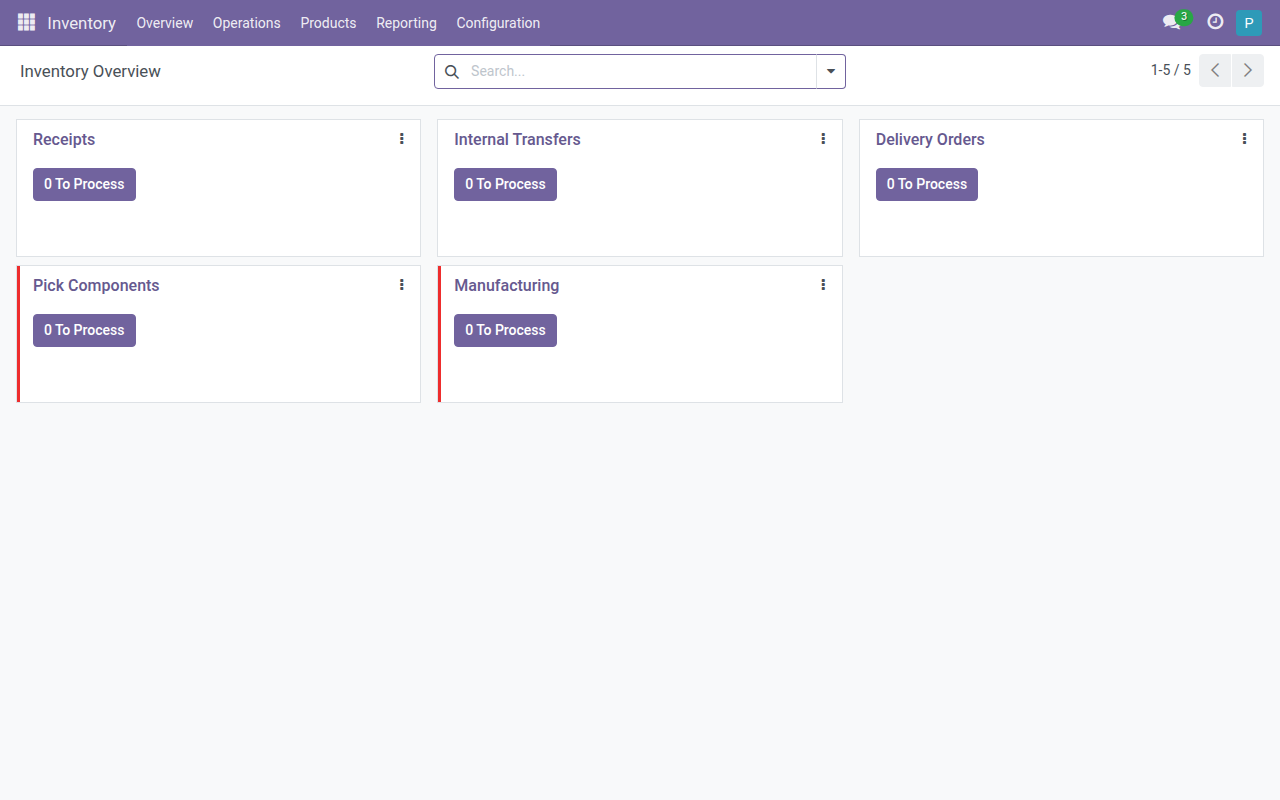
\includegraphics[width=0.9\textwidth]{manual/images/supplychain/01_inventory_dashboard.png}
    \caption{Inventory Dashboard showing the initial state.}
\end{figure}

% ============================================================
% STEP 2: CREATING A PURCHASE ORDER
% ============================================================
\section{Step 2: Creating a Purchase Order (PO)}

If the requested material is out of stock, we must order it from our supplier.

\begin{enumerate}
    \item Open the \textbf{Purchase} application from the main dashboard.
    \item Click the \textbf{New} button to create a Request for Quotation (RFQ).
    \item Under the \textbf{Vendor} field, type the name of the supplier (e.g., \textit{Dazzle Robotics}).
    \item Under the \textbf{Products} tab, click \textbf{Add a product} and select the required material.
    \item Enter the quantity and unit price. Click \textbf{Save}.
\end{enumerate}

\begin{figure}[H]
    \centering
    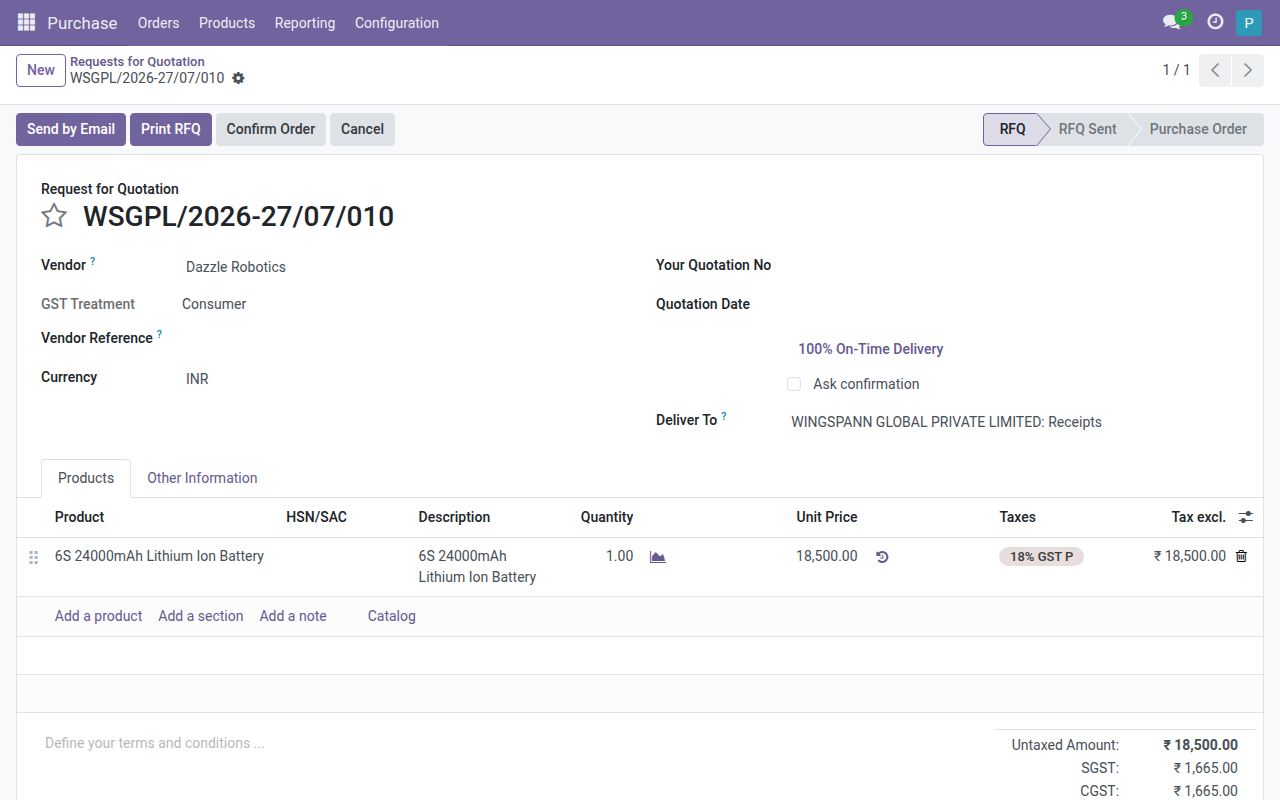
\includegraphics[width=0.9\textwidth]{manual/images/supplychain/02_po_draft.png}
    \caption{A new Draft Purchase Order with vendor and product selected.}
\end{figure}

% ============================================================
% STEP 3: CONFIRMING AND PRINTING THE PO
% ============================================================
\section{Step 3: Confirming and Printing the PO}

Once the details are finalized, it is time to formally confirm the purchase order. This locks in the prices and notifies the system that a delivery is expected.

\begin{enumerate}
    \item On the Purchase Order page, click the \textbf{Confirm Order} button. 
    \item The status will change from RFQ to \textbf{Purchase Order}.
    \item Click the \textbf{Print} icon at the top and select \textbf{Purchase Order} to generate the PDF.
\end{enumerate}

\begin{warnbox}
If the Purchase Order exceeds a certain monetary limit, it may require Manager Approval before it becomes confirmed. The manager will be notified automatically.
\end{warnbox}

\begin{figure}[H]
    \centering
    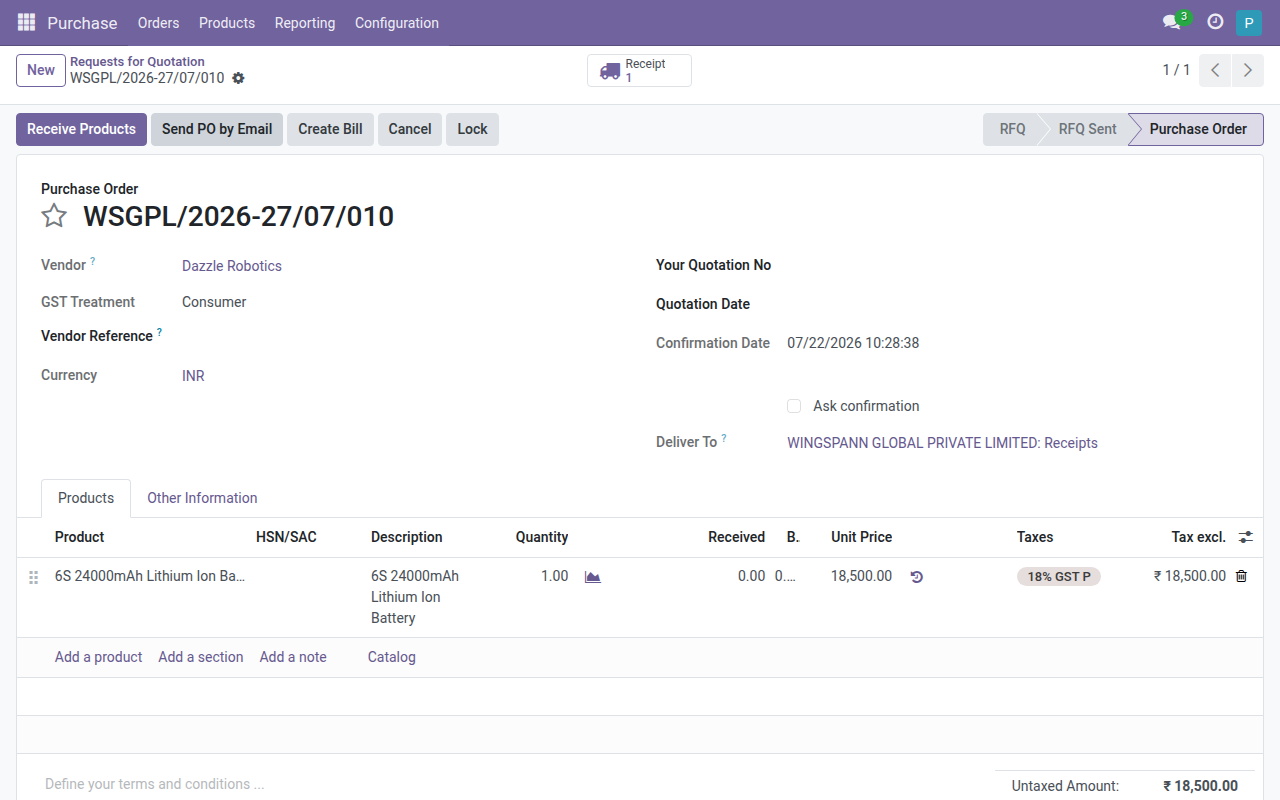
\includegraphics[width=0.9\textwidth]{manual/images/supplychain/04_po_confirmed.png}
    \caption{The Purchase Order has been confirmed.}
\end{figure}

Below is the visual format of the printed Purchase Order document which is sent to the supplier:

\begin{figure}[H]
    \centering
    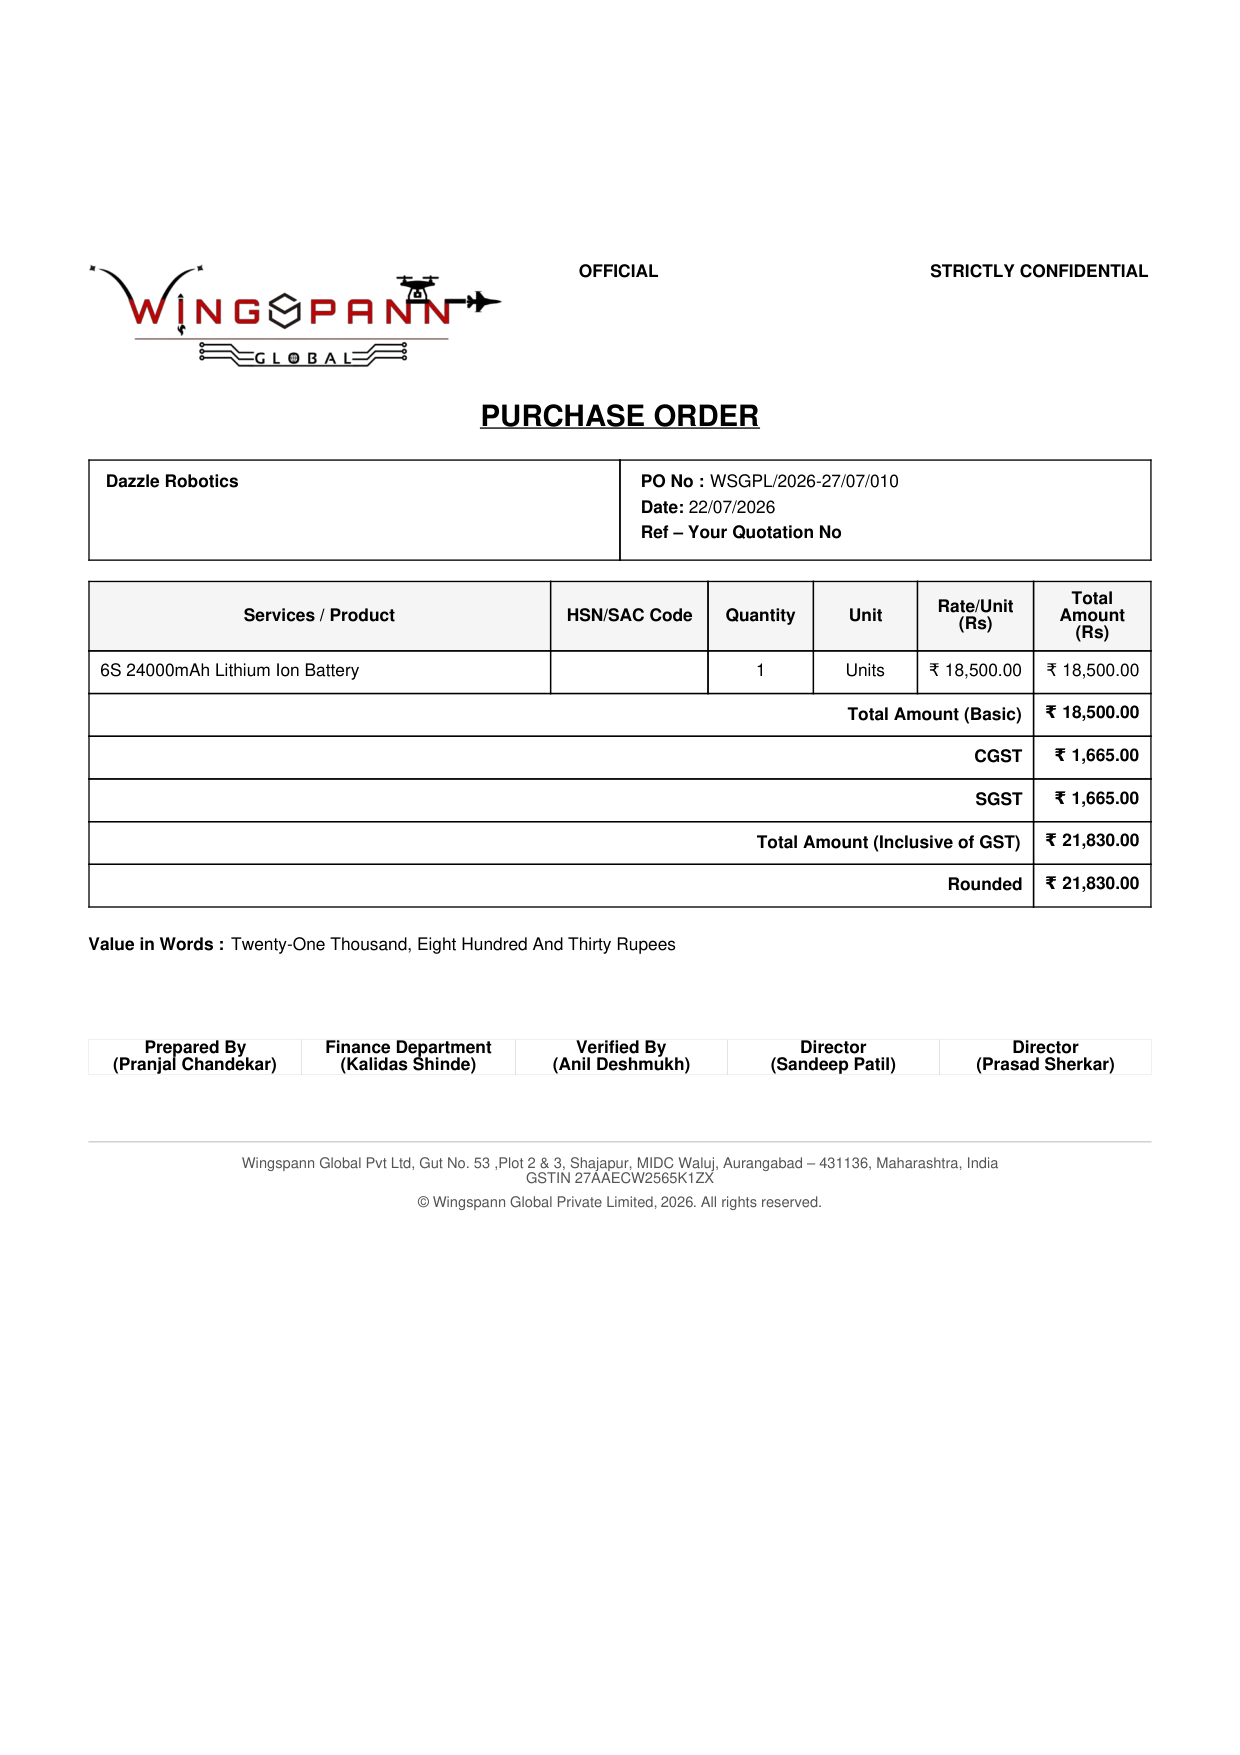
\includegraphics[width=0.8\textwidth]{manual/images/supplychain/03_po_document.png}
    \caption{The Generated Purchase Order PDF Document.}
\end{figure}

% ============================================================
% STEP 4: RECEIVING THE GOODS
% ============================================================
\section{Step 4: Receiving the Goods}

When the physical goods arrive at our warehouse, the inventory must be updated so the manufacturer can finally use the items.

\begin{enumerate}
    \item From your confirmed Purchase Order, look for the \textbf{Receipt} smart button in the top right corner and click it. (Alternatively, go to the Inventory app and click Receipts).
    \item You will see a list of the expected items. Ensure the physical quantity received matches what is on the screen.
    \item Click \textbf{Validate} to officially bring the items into our stock.
\end{enumerate}

\begin{figure}[H]
    \centering
    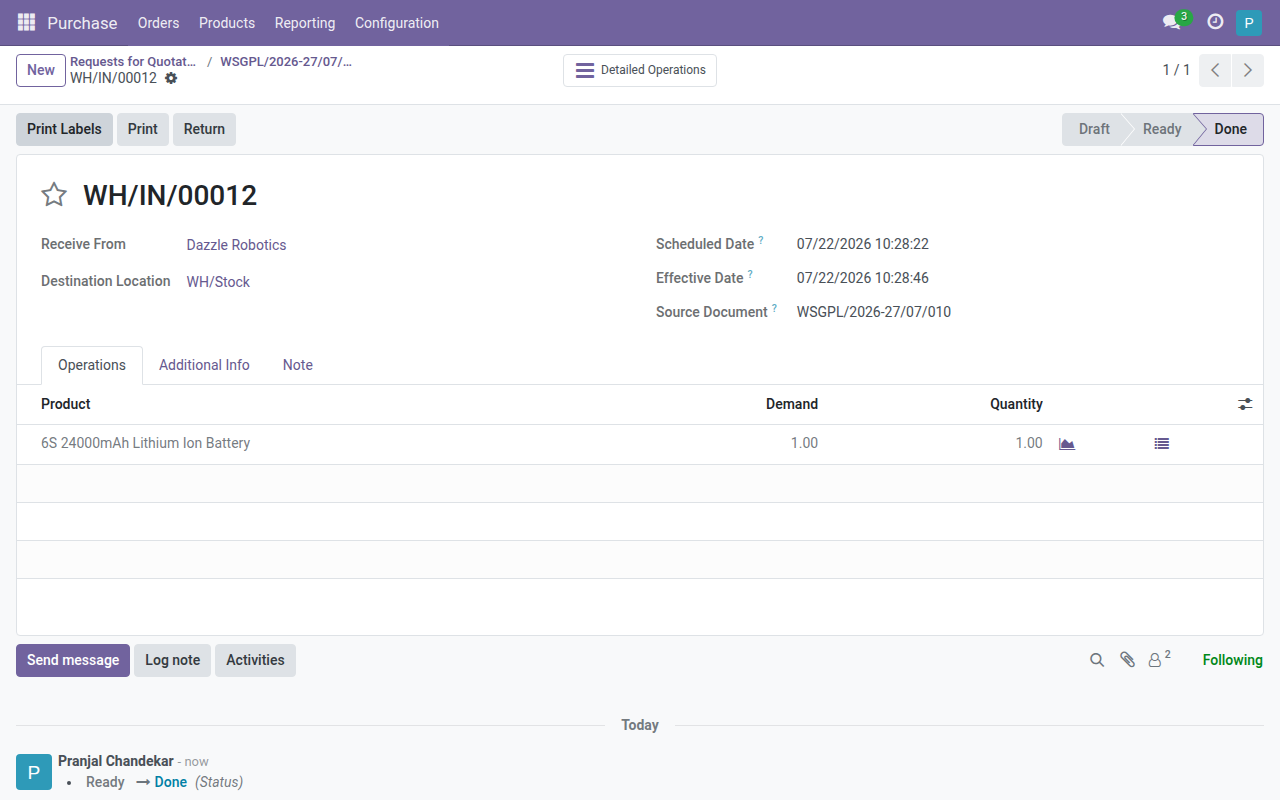
\includegraphics[width=0.9\textwidth]{manual/images/supplychain/05_receipt_validated.png}
    \caption{The Receipt has been successfully validated and the inventory is updated.}
\end{figure}

% ============================================================
% STEP 5: CREATING THE VENDOR BILL FOR FINANCE
% ============================================================
\section{Step 5: Creating the Vendor Bill for Finance}

Now that the goods are received (or sometimes, if advance payment is required, before the goods arrive), you must create a Vendor Bill to pass onto the Finance team for payment approval.

\begin{enumerate}
    \item Go back to your confirmed Purchase Order.
    \item Click the \textbf{Create Bill} button at the top.
    \item A draft bill will be generated. Fill in the \textbf{Bill Date} with today's date.
    \item Click \textbf{Confirm}. The bill is now official and will be queued up for the Finance Officer to review and pay.
\end{enumerate}

\begin{figure}[H]
    \centering
    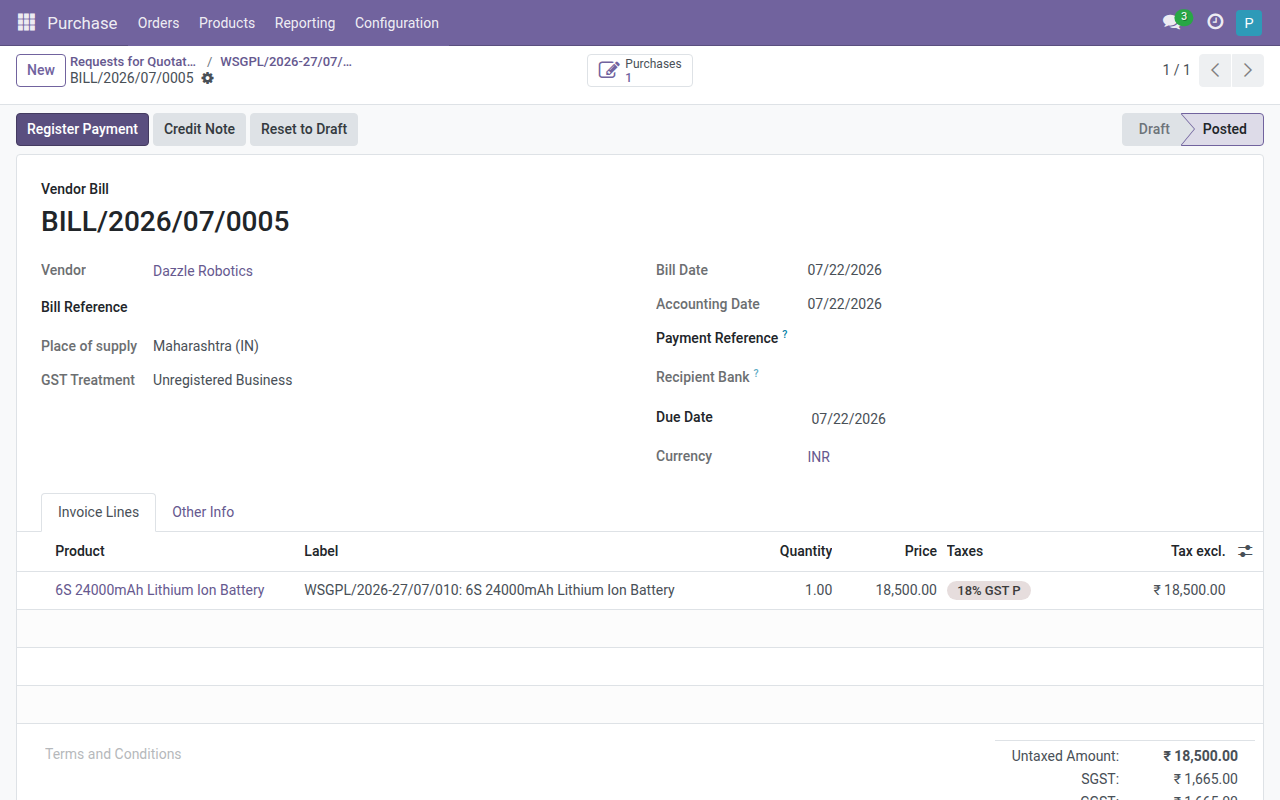
\includegraphics[width=0.9\textwidth]{manual/images/supplychain/07_vendor_bill_confirmed.png}
    \caption{The Vendor Bill is confirmed and ready for Finance.}
\end{figure}


Below is the printed Tax Invoice (Bill) document that is generated at this stage:

\begin{figure}[H]
    \centering
    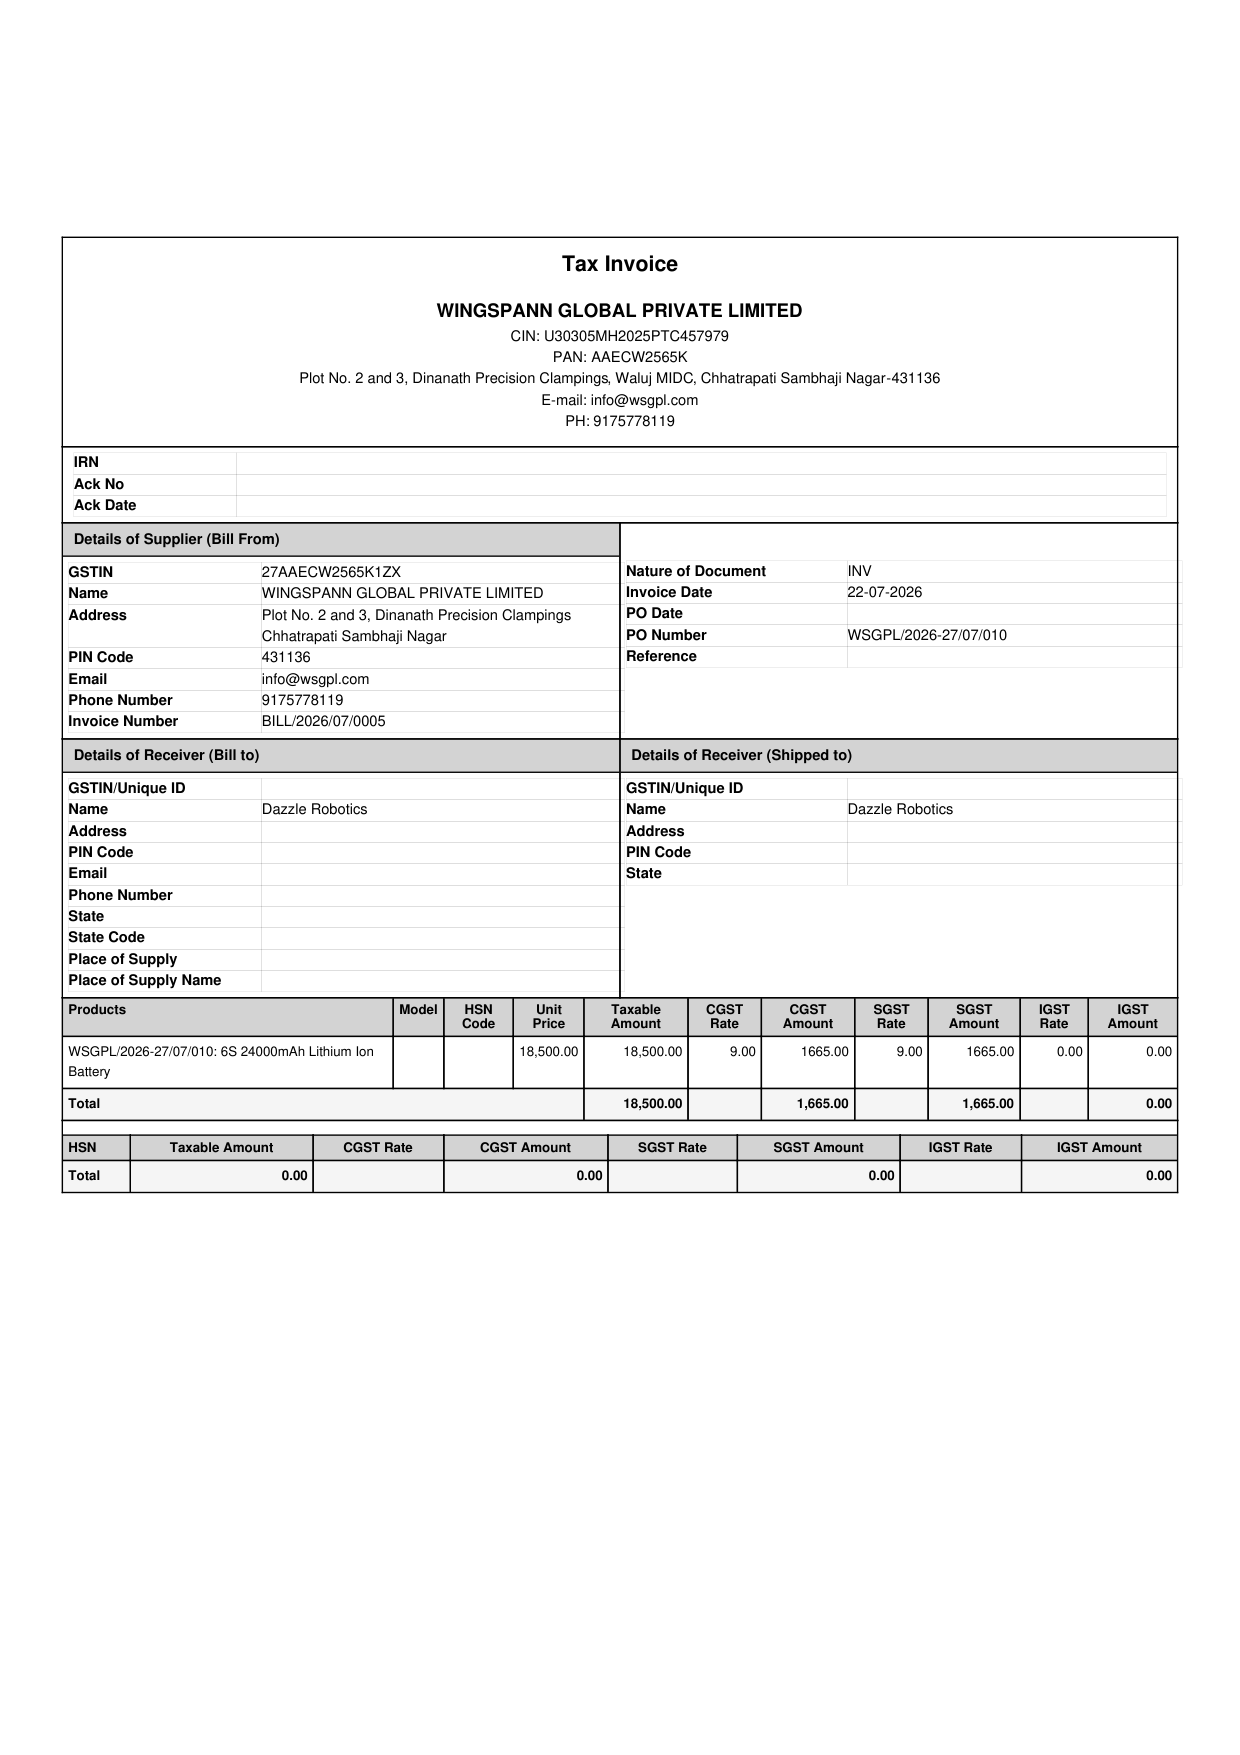
\includegraphics[width=0.8\textwidth]{manual/images/supplychain/08_bill_document.png}
    \caption{The Generated Vendor Bill (Tax Invoice) PDF Document.}
\end{figure}

\end{document}
